\chapter{Benchmarking tables}
\label{chap:benchmarking-tables}

This appendix contains the full tables with memory benchmarking results and
phrase table sizes obtained by the procedure described in \Sref{sec:memory-benchmarking}.

Figures below display a graphical overview of the virtual memory peaks measured on the Cs-En setup
(\Fref{fig:cs-en-vm-peaks-summary}) and the Fr-En setup (\Fref{fig:fr-en-vm-peaks-summary}).

\begin{figure}[!htb]
  \centering
  % GNUPLOT: LaTeX picture with Postscript
\begingroup
  \makeatletter
  \providecommand\color[2][]{%
    \GenericError{(gnuplot) \space\space\space\@spaces}{%
      Package color not loaded in conjunction with
      terminal option `colourtext'%
    }{See the gnuplot documentation for explanation.%
    }{Either use 'blacktext' in gnuplot or load the package
      color.sty in LaTeX.}%
    \renewcommand\color[2][]{}%
  }%
  \providecommand\includegraphics[2][]{%
    \GenericError{(gnuplot) \space\space\space\@spaces}{%
      Package graphicx or graphics not loaded%
    }{See the gnuplot documentation for explanation.%
    }{The gnuplot epslatex terminal needs graphicx.sty or graphics.sty.}%
    \renewcommand\includegraphics[2][]{}%
  }%
  \providecommand\rotatebox[2]{#2}%
  \@ifundefined{ifGPcolor}{%
    \newif\ifGPcolor
    \GPcolorfalse
  }{}%
  \@ifundefined{ifGPblacktext}{%
    \newif\ifGPblacktext
    \GPblacktexttrue
  }{}%
  % define a \g@addto@macro without @ in the name:
  \let\gplgaddtomacro\g@addto@macro
  % define empty templates for all commands taking text:
  \gdef\gplbacktext{}%
  \gdef\gplfronttext{}%
  \makeatother
  \ifGPblacktext
    % no textcolor at all
    \def\colorrgb#1{}%
    \def\colorgray#1{}%
  \else
    % gray or color?
    \ifGPcolor
      \def\colorrgb#1{\color[rgb]{#1}}%
      \def\colorgray#1{\color[gray]{#1}}%
      \expandafter\def\csname LTw\endcsname{\color{white}}%
      \expandafter\def\csname LTb\endcsname{\color{black}}%
      \expandafter\def\csname LTa\endcsname{\color{black}}%
      \expandafter\def\csname LT0\endcsname{\color[rgb]{1,0,0}}%
      \expandafter\def\csname LT1\endcsname{\color[rgb]{0,1,0}}%
      \expandafter\def\csname LT2\endcsname{\color[rgb]{0,0,1}}%
      \expandafter\def\csname LT3\endcsname{\color[rgb]{1,0,1}}%
      \expandafter\def\csname LT4\endcsname{\color[rgb]{0,1,1}}%
      \expandafter\def\csname LT5\endcsname{\color[rgb]{1,1,0}}%
      \expandafter\def\csname LT6\endcsname{\color[rgb]{0,0,0}}%
      \expandafter\def\csname LT7\endcsname{\color[rgb]{1,0.3,0}}%
      \expandafter\def\csname LT8\endcsname{\color[rgb]{0.5,0.5,0.5}}%
    \else
      % gray
      \def\colorrgb#1{\color{black}}%
      \def\colorgray#1{\color[gray]{#1}}%
      \expandafter\def\csname LTw\endcsname{\color{white}}%
      \expandafter\def\csname LTb\endcsname{\color{black}}%
      \expandafter\def\csname LTa\endcsname{\color{black}}%
      \expandafter\def\csname LT0\endcsname{\color{black}}%
      \expandafter\def\csname LT1\endcsname{\color{black}}%
      \expandafter\def\csname LT2\endcsname{\color{black}}%
      \expandafter\def\csname LT3\endcsname{\color{black}}%
      \expandafter\def\csname LT4\endcsname{\color{black}}%
      \expandafter\def\csname LT5\endcsname{\color{black}}%
      \expandafter\def\csname LT6\endcsname{\color{black}}%
      \expandafter\def\csname LT7\endcsname{\color{black}}%
      \expandafter\def\csname LT8\endcsname{\color{black}}%
    \fi
  \fi
  \setlength{\unitlength}{0.0500bp}%
  \begin{picture}(6480.00,4536.00)%
    \gplgaddtomacro\gplbacktext{%
      \csname LTb\endcsname%
      \put(814,704){\makebox(0,0)[r]{\strut{} 0}}%
      \put(814,1100){\makebox(0,0)[r]{\strut{} 5}}%
      \put(814,1497){\makebox(0,0)[r]{\strut{} 10}}%
      \put(814,1893){\makebox(0,0)[r]{\strut{} 15}}%
      \put(814,2290){\makebox(0,0)[r]{\strut{} 20}}%
      \put(814,2686){\makebox(0,0)[r]{\strut{} 25}}%
      \put(814,3082){\makebox(0,0)[r]{\strut{} 30}}%
      \put(814,3479){\makebox(0,0)[r]{\strut{} 35}}%
      \put(814,3875){\makebox(0,0)[r]{\strut{} 40}}%
      \put(946,484){\makebox(0,0){\strut{} 0}}%
      \put(1588,484){\makebox(0,0){\strut{} 2}}%
      \put(2230,484){\makebox(0,0){\strut{} 4}}%
      \put(2872,484){\makebox(0,0){\strut{} 6}}%
      \put(3515,484){\makebox(0,0){\strut{} 8}}%
      \put(4157,484){\makebox(0,0){\strut{} 10}}%
      \put(4799,484){\makebox(0,0){\strut{} 12}}%
      \put(5441,484){\makebox(0,0){\strut{} 14}}%
      \put(6083,484){\makebox(0,0){\strut{} 16}}%
      \put(176,2289){\rotatebox{-270}{\makebox(0,0){\strut{}virtual memory peak (GB)}}}%
      \put(3514,154){\makebox(0,0){\strut{}input size in sentences (M)}}%
      \put(3514,4205){\makebox(0,0){\strut{}Cs-En: corpus size vs. VM peak}}%
    }%
    \gplgaddtomacro\gplfronttext{%
      \csname LTb\endcsname%
      \put(2530,3702){\makebox(0,0)[r]{\strut{}eppex zero}}%
      \csname LTb\endcsname%
      \put(2530,3482){\makebox(0,0)[r]{\strut{}eppex def.}}%
      \csname LTb\endcsname%
      \put(2530,3262){\makebox(0,0)[r]{\strut{}eppex 0:n}}%
      \csname LTb\endcsname%
      \put(2530,3042){\makebox(0,0)[r]{\strut{}eppex 0:n+1}}%
      \csname LTb\endcsname%
      \put(2530,2822){\makebox(0,0)[r]{\strut{}eppex 1:n+1}}%
    }%
    \gplbacktext
    \put(0,0){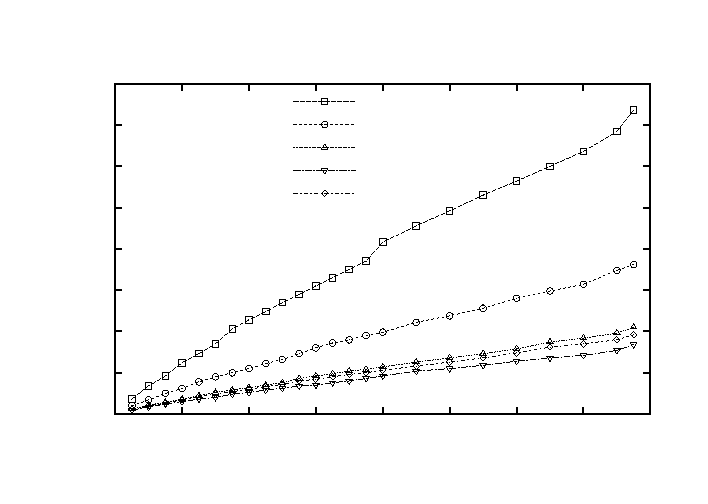
\includegraphics{summary-cs-en-vm-peaks}}%
    \gplfronttext
  \end{picture}%
\endgroup

  \caption{
    A plot of the virtual memory peaks of several \eppex{} configurations invoked on subsets of the Cs-En training data.
  }
  \label{fig:cs-en-vm-peaks-summary}
\end{figure}

\begin{figure}[!htb]
  \centering
  % GNUPLOT: LaTeX picture with Postscript
\begingroup
  \makeatletter
  \providecommand\color[2][]{%
    \GenericError{(gnuplot) \space\space\space\@spaces}{%
      Package color not loaded in conjunction with
      terminal option `colourtext'%
    }{See the gnuplot documentation for explanation.%
    }{Either use 'blacktext' in gnuplot or load the package
      color.sty in LaTeX.}%
    \renewcommand\color[2][]{}%
  }%
  \providecommand\includegraphics[2][]{%
    \GenericError{(gnuplot) \space\space\space\@spaces}{%
      Package graphicx or graphics not loaded%
    }{See the gnuplot documentation for explanation.%
    }{The gnuplot epslatex terminal needs graphicx.sty or graphics.sty.}%
    \renewcommand\includegraphics[2][]{}%
  }%
  \providecommand\rotatebox[2]{#2}%
  \@ifundefined{ifGPcolor}{%
    \newif\ifGPcolor
    \GPcolorfalse
  }{}%
  \@ifundefined{ifGPblacktext}{%
    \newif\ifGPblacktext
    \GPblacktexttrue
  }{}%
  % define a \g@addto@macro without @ in the name:
  \let\gplgaddtomacro\g@addto@macro
  % define empty templates for all commands taking text:
  \gdef\gplbacktext{}%
  \gdef\gplfronttext{}%
  \makeatother
  \ifGPblacktext
    % no textcolor at all
    \def\colorrgb#1{}%
    \def\colorgray#1{}%
  \else
    % gray or color?
    \ifGPcolor
      \def\colorrgb#1{\color[rgb]{#1}}%
      \def\colorgray#1{\color[gray]{#1}}%
      \expandafter\def\csname LTw\endcsname{\color{white}}%
      \expandafter\def\csname LTb\endcsname{\color{black}}%
      \expandafter\def\csname LTa\endcsname{\color{black}}%
      \expandafter\def\csname LT0\endcsname{\color[rgb]{1,0,0}}%
      \expandafter\def\csname LT1\endcsname{\color[rgb]{0,1,0}}%
      \expandafter\def\csname LT2\endcsname{\color[rgb]{0,0,1}}%
      \expandafter\def\csname LT3\endcsname{\color[rgb]{1,0,1}}%
      \expandafter\def\csname LT4\endcsname{\color[rgb]{0,1,1}}%
      \expandafter\def\csname LT5\endcsname{\color[rgb]{1,1,0}}%
      \expandafter\def\csname LT6\endcsname{\color[rgb]{0,0,0}}%
      \expandafter\def\csname LT7\endcsname{\color[rgb]{1,0.3,0}}%
      \expandafter\def\csname LT8\endcsname{\color[rgb]{0.5,0.5,0.5}}%
    \else
      % gray
      \def\colorrgb#1{\color{black}}%
      \def\colorgray#1{\color[gray]{#1}}%
      \expandafter\def\csname LTw\endcsname{\color{white}}%
      \expandafter\def\csname LTb\endcsname{\color{black}}%
      \expandafter\def\csname LTa\endcsname{\color{black}}%
      \expandafter\def\csname LT0\endcsname{\color{black}}%
      \expandafter\def\csname LT1\endcsname{\color{black}}%
      \expandafter\def\csname LT2\endcsname{\color{black}}%
      \expandafter\def\csname LT3\endcsname{\color{black}}%
      \expandafter\def\csname LT4\endcsname{\color{black}}%
      \expandafter\def\csname LT5\endcsname{\color{black}}%
      \expandafter\def\csname LT6\endcsname{\color{black}}%
      \expandafter\def\csname LT7\endcsname{\color{black}}%
      \expandafter\def\csname LT8\endcsname{\color{black}}%
    \fi
  \fi
  \setlength{\unitlength}{0.0500bp}%
  \begin{picture}(6480.00,4536.00)%
    \gplgaddtomacro\gplbacktext{%
      \csname LTb\endcsname%
      \put(946,704){\makebox(0,0)[r]{\strut{} 0}}%
      \put(946,1425){\makebox(0,0)[r]{\strut{} 50}}%
      \put(946,2145){\makebox(0,0)[r]{\strut{} 100}}%
      \put(946,2866){\makebox(0,0)[r]{\strut{} 150}}%
      \put(946,3587){\makebox(0,0)[r]{\strut{} 200}}%
      \put(1078,484){\makebox(0,0){\strut{} 0}}%
      \put(1704,484){\makebox(0,0){\strut{} 5}}%
      \put(2329,484){\makebox(0,0){\strut{} 10}}%
      \put(2955,484){\makebox(0,0){\strut{} 15}}%
      \put(3581,484){\makebox(0,0){\strut{} 20}}%
      \put(4206,484){\makebox(0,0){\strut{} 25}}%
      \put(4832,484){\makebox(0,0){\strut{} 30}}%
      \put(5457,484){\makebox(0,0){\strut{} 35}}%
      \put(6083,484){\makebox(0,0){\strut{} 40}}%
      \put(176,2289){\rotatebox{-270}{\makebox(0,0){\strut{}virtual memory peak (GB)}}}%
      \put(3580,154){\makebox(0,0){\strut{}input size in sentences (M)}}%
      \put(3580,4205){\makebox(0,0){\strut{}Fr-En: corpus size vs. VM peak}}%
    }%
    \gplgaddtomacro\gplfronttext{%
      \csname LTb\endcsname%
      \put(2662,3702){\makebox(0,0)[r]{\strut{}eppex zero}}%
      \csname LTb\endcsname%
      \put(2662,3482){\makebox(0,0)[r]{\strut{}eppex def.}}%
      \csname LTb\endcsname%
      \put(2662,3262){\makebox(0,0)[r]{\strut{}eppex 0:n}}%
      \csname LTb\endcsname%
      \put(2662,3042){\makebox(0,0)[r]{\strut{}eppex 1:n+1}}%
      \csname LTb\endcsname%
      \put(2662,2822){\makebox(0,0)[r]{\strut{}eppex 1:n+2}}%
    }%
    \gplbacktext
    \put(0,0){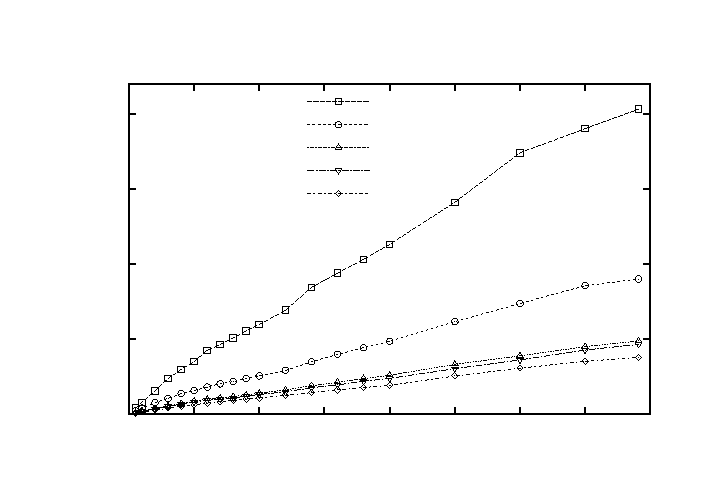
\includegraphics{summary-fr-en-vm-peaks}}%
    \gplfronttext
  \end{picture}%
\endgroup

  \caption{
    A plot of the virtual memory peaks of several \eppex{} configurations invoked on subsets of the Fr-En training data.
  }
  \label{fig:fr-en-vm-peaks-summary}
\end{figure}

\openright
\section{Cs-En dataset}

% Memory benchmarking table for Cs-En
\begin{table}[!htb]
\centering
\def\arraystretch{1.1}
\begin{tabular}{ | r  r  r | r  r  r  r  r | }
\hline
\multicolumn{3}{|c|}{input data size} & \multicolumn{5}{|c|}{virtual memory peak per eppex configuration} \\
sent. & source & target & zero & def. & 0:n & 0:n+1 & 1:n+1 \\
\hline
\hline
0.1~M & 1.4~M & 1.6~M & 467~MB & 268~MB & 187~MB & 171~MB & 151~MB \\
0.2~M & 2.8~M & 3.2~M & 856~MB & 478~MB & 297~MB & 263~MB & 278~MB \\
0.3~M & 4.1~M & 4.8~M & 1.2~GB & 649~MB & 398~MB & 355~MB & 371~MB \\
0.4~M & 5.5~M & 6.3~M & 1.5~GB & 799~MB & 495~MB & 424~MB & 460~MB \\
0.5~M & 6.9~M & 7.9~M & 1.8~GB & 1.0~GB & 599~MB & 492~MB & 557~MB \\
0.6~M & 8.3~M & 9.5~M & 2.1~GB & 1.2~GB & 704~MB & 561~MB & 654~MB \\
0.7~M & 9.7~M & 11.1~M & 2.6~GB & 1.3~GB & 814~MB & 646~MB & 757~MB \\
0.8~M & 11.1~M & 12.7~M & 2.9~GB & 1.4~GB & 897~MB & 731~MB & 834~MB \\
0.9~M & 12.5~M & 14.3~M & 3.1~GB & 1.6~GB & 1.0~GB & 805~MB & 932~MB \\
1.0~M & 13.8~M & 15.9~M & 3.4~GB & 1.7~GB & 1.1~GB & 861~MB & 1.0~GB \\
1.5~M & 20.7~M & 23.8~M & 4.6~GB & 2.5~GB & 1.4~GB & 1.2~GB & 1.3~GB \\
2.0~M & 27.6~M & 31.8~M & 6.2~GB & 3.1~GB & 1.8~GB & 1.5~GB & 1.7~GB \\
2.5~M & 34.6~M & 39.7~M & 7.3~GB & 3.9~GB & 2.2~GB & 1.8~GB & 2.1~GB \\
3.0~M & 41.5~M & 47.7~M & 8.5~GB & 4.5~GB & 2.6~GB & 2.0~GB & 2.4~GB \\
3.5~M & 48.4~M & 55.6~M & 10.3~GB & 5.0~GB & 2.9~GB & 2.4~GB & 2.7~GB \\
4.0~M & 55.3~M & 63.5~M & 11.4~GB & 5.5~GB & 3.2~GB & 2.6~GB & 3.0~GB \\
4.5~M & 62.2~M & 71.5~M & 12.4~GB & 6.1~GB & 3.5~GB & 2.9~GB & 3.3~GB \\
5.0~M & 69.1~M & 79.4~M & 13.5~GB & 6.6~GB & 3.8~GB & 3.1~GB & 3.6~GB \\
5.5~M & 76.0~M & 87.3~M & 14.5~GB & 7.3~GB & 4.3~GB & 3.4~GB & 4.0~GB \\
6.0~M & 82.9~M & 95.2~M & 15.5~GB & 8.0~GB & 4.6~GB & 3.5~GB & 4.2~GB \\
6.5~M & 89.8~M & 103~M & 16.5~GB & 8.6~GB & 4.9~GB & 3.8~GB & 4.5~GB \\
7.0~M & 96.8~M & 111~M & 17.5~GB & 9.0~GB & 5.2~GB & 4.0~GB & 4.8~GB \\
7.5~M & 104~M & 119~M & 18.5~GB & 9.5~GB & 5.4~GB & 4.3~GB & 5.0~GB \\
8.0~M & 111~M & 127~M & 20.8~GB & 9.9~GB & 5.7~GB & 4.6~GB & 5.3~GB \\
9.0~M & 124~M & 143~M & 22.8~GB & 11.1~GB & 6.3~GB & 5.2~GB & 5.8~GB \\
10~M & 138~M & 159~M & 24.6~GB & 11.9~GB & 6.8~GB & 5.5~GB & 6.3~GB \\
11~M & 152~M & 175~M & 26.5~GB & 12.8~GB & 7.3~GB & 5.9~GB & 6.8~GB \\
12~M & 166~M & 191~M & 28.2~GB & 14.0~GB & 7.9~GB & 6.4~GB & 7.4~GB \\
13~M & 180~M & 206~M & 30.0~GB & 14.9~GB & 8.7~GB & 6.8~GB & 8.1~GB \\
14~M & 194~M & 222~M & 31.8~GB & 15.7~GB & 9.2~GB & 7.1~GB & 8.5~GB \\
15~M & 209~M & 240~M & 34.2~GB & 17.4~GB & 9.8~GB & 7.7~GB & 9.0~GB \\
full & 220~M & 253~M & 36.8~GB & 18.1~GB & 10.5~GB & 8.4~GB & 9.6~GB \\
\hline
\end{tabular}
\caption{\label{cs-en-memory-benchmarking}
Virtual memory peaks of the phrase table construction performed with
various configurations of \eppex{} run on portions of Cs-En dataset.
The input data size triple stands for: number of parallel sentences and number of words on the source and target side.
The full corpus had almost 15.5~M of parallel sentences.}
\end{table}

% Output size benchmarking table for Cs-En
\begin{table}[!htb]
\centering
\def\arraystretch{1.1}
\begin{tabular}{ | r  r  r | r  r  r  r  r | }
\hline
\multicolumn{3}{|c|}{input data size} & \multicolumn{5}{|c|}{phrase table size per eppex configuration} \\
sent. & source & target & zero & def. & 0:n & 0:n+1 & 1:n+1 \\
\hline
\hline
0.1~M & 1.4~M & 1.6~M & 3.6~M & 1.5~M & 853~K & 590~K & 187~K \\
0.2~M & 2.8~M & 3.2~M & 6.9~M & 2.7~M & 1.6~M & 1.2~M & 381~K \\
0.3~M & 4.1~M & 4.8~M & 10.0~M & 3.8~M & 2.4~M & 1.7~M & 567~K \\
0.4~M & 5.5~M & 6.3~M & 13.0~M & 4.9~M & 3.1~M & 2.2~M & 759~K \\
0.5~M & 6.9~M & 7.9~M & 15.9~M & 6.0~M & 3.8~M & 2.7~M & 958~K \\
0.6~M & 8.3~M & 9.5~M & 18.7~M & 7.0~M & 4.4~M & 3.2~M & 1.2~M \\
0.7~M & 9.7~M & 11.1~M & 21.5~M & 8.0~M & 5.1~M & 3.7~M & 1.4~M \\
0.8~M & 11.1~M & 12.7~M & 24.1~M & 9.0~M & 5.7~M & 4.1~M & 1.6~M \\
0.9~M & 12.5~M & 14.3~M & 26.7~M & 10.0~M & 6.3~M & 4.6~M & 1.8~M \\
1.0~M & 13.8~M & 15.9~M & 29.3~M & 10.9~M & 7.0~M & 5.1~M & 2.0~M \\
1.5~M & 20.7~M & 23.8~M & 41.8~M & 15.4~M & 10.0~M & 7.5~M & 3.1~M \\
2.0~M & 27.6~M & 31.8~M & 53.7~M & 19.6~M & 12.9~M & 9.7~M & 4.0~M \\
2.5~M & 34.6~M & 39.7~M & 65.3~M & 23.7~M & 15.7~M & 11.8~M & 5.0~M \\
3.0~M & 41.5~M & 47.7~M & 76.5~M & 27.6~M & 18.3~M & 13.9~M & 5.9~M \\
3.5~M & 48.4~M & 55.6~M & 87.4~M & 31.3~M & 20.9~M & 15.9~M & 6.8~M \\
4.0~M & 55.3~M & 63.5~M & 98.1~M & 34.9~M & 23.2~M & 17.7~M & 7.5~M \\
4.5~M & 62.2~M & 71.5~M & 109~M & 38.4~M & 25.7~M & 19.6~M & 8.3~M \\
5.0~M & 69.1~M & 79.4~M & 119~M & 41.9~M & 28.1~M & 21.4~M & 9.1~M \\
5.5~M & 76.0~M & 87.3~M & 129~M & 45.2~M & 30.4~M & 23.2~M & 9.8~M \\
6.0~M & 82.9~M & 95.2~M & 139~M & 48.5~M & 32.7~M & 25.0~M & 10.5~M \\
6.5~M & 89.8~M & 103~M & 149~M & 51.7~M & 34.9~M & 26.6~M & 11.3~M \\
7.0~M & 96.8~M & 111~M & 159~M & 54.9~M & 37.2~M & 28.3~M & 12.0~M \\
7.5~M & 104~M & 119~M & 169~M & 58.1~M & 39.4~M & 30.1~M & 12.7~M \\
8.0~M & 111~M & 127~M & 179~M & 61.2~M & 41.7~M & 31.9~M & 13.4~M \\
9.0~M & 124~M & 143~M & 198~M & 67.3~M & 46.2~M & 35.3~M & 14.9~M \\
10~M & 138~M & 159~M & 216~M & 73.3~M & 50.5~M & 38.6~M & 16.4~M \\
11~M & 152~M & 175~M & 234~M & 79.2~M & 54.7~M & 41.9~M & 17.9~M \\
12~M & 166~M & 191~M & 252~M & 84.9~M & 59.0~M & 45.2~M & 19.4~M \\
13~M & 180~M & 206~M & 269~M & 90.6~M & 63.2~M & 48.5~M & 20.9~M \\
14~M & 194~M & 222~M & 287~M & 96.2~M & 67.3~M & 51.7~M & 22.4~M \\
15~M & 209~M & 240~M & 310~M & 103~M & 75.1~M & 58.3~M & 24.0~M \\
full & 220~M & 253~M & 336~M & 110~M & 86.2~M & 67.9~M & 25.7~M \\
\hline
\end{tabular}
\caption{\label{cs-en-output-size-benchmarking}
Phrase table sizes (in phrase pairs) obtained with various configurations of \eppex{}
on portions of Cs-En dataset. The input data size triple stands for: number of
parallel sentences and number of words on the source and target side.
The full corpus had almost 15.5~M of parallel sentences.}
\end{table}

\openright
\section{Fr-En dataset}

% Memory benchmarking table for Fr-En
\begin{table}[!htb]
\centering
\def\arraystretch{1.1}
\begin{tabular}{ | r  r  r | r  r  r  r  r | }
\hline
\multicolumn{3}{|c|}{input data size} & \multicolumn{5}{|c|}{virtual memory peak per eppex configuration} \\
sent. & source & target & zero & def. & zero-n & 1:n+1 & 1:n+2 \\
\hline
\hline
.1~M & 2.6~M & 2.4~M & 0.9~GB & 0.4~GB & 0.3~GB & 0.2~GB & 0.2~GB \\
.2~M & 5.1~M & 4.8~M & 1.7~GB & 0.8~GB & 0.4~GB & 0.4~GB & 0.3~GB \\
.3~M & 7.7~M & 7.2~M & 2.5~GB & 1.2~GB & 0.6~GB & 0.6~GB & 0.5~GB \\
.4~M & 10.2~M & 9.6~M & 3.2~GB & 1.5~GB & 0.8~GB & 0.8~GB & 0.6~GB \\
.5~M & 12.8~M & 12.1~M & 4.0~GB & 2.0~GB & 1.0~GB & 0.9~GB & 0.7~GB \\
.6~M & 15.5~M & 14.5~M & 5.0~GB & 2.3~GB & 1.2~GB & 1.1~GB & 0.9~GB \\
.7~M & 18.2~M & 16.9~M & 5.7~GB & 2.6~GB & 1.4~GB & 1.3~GB & 1.0~GB \\
.8~M & 21.0~M & 19.3~M & 6.4~GB & 3.0~GB & 1.6~GB & 1.4~GB & 1.2~GB \\
.9~M & 23.7~M & 21.8~M & 7.1~GB & 3.4~GB & 1.8~GB & 1.7~GB & 1.3~GB \\
1~M & 26.6~M & 24.3~M & 7.8~GB & 3.8~GB & 2.0~GB & 1.8~GB & 1.4~GB \\
2~M & 53.6~M & 48.4~M & 15.4~GB & 7.4~GB & 3.8~GB & 3.4~GB & 2.6~GB \\
3~M & 80.2~M & 72.3~M & 23.6~GB & 10.4~GB & 5.5~GB & 5.0~GB & 3.9~GB \\
4~M & 109~M & 98.8~M & 29.7~GB & 13.6~GB & 7.0~GB & 6.5~GB & 5.1~GB \\
5~M & 138~M & 125~M & 35.0~GB & 15.7~GB & 8.5~GB & 7.9~GB & 6.2~GB \\
6~M & 166~M & 148~M & 42.4~GB & 18.0~GB & 9.8~GB & 9.1~GB & 7.3~GB \\
7~M & 193~M & 171~M & 46.3~GB & 20.1~GB & 10.7~GB & 10.1~GB & 8.1~GB \\
8~M & 222~M & 195~M & 50.8~GB & 21.6~GB & 11.6~GB & 10.8~GB & 9.1~GB \\
9~M & 251~M & 219~M & 55.3~GB & 23.7~GB & 12.6~GB & 11.8~GB & 9.9~GB \\
10~M & 279~M & 242~M & 59.6~GB & 25.4~GB & 13.9~GB & 13.0~GB & 10.6~GB \\
12~M & 338~M & 291~M & 69.1~GB & 29.1~GB & 16.0~GB & 14.8~GB & 12.4~GB \\
14~M & 398~M & 341~M & 84.3~GB & 34.8~GB & 18.9~GB & 17.5~GB & 14.2~GB \\
16~M & 458~M & 391~M & 93.8~GB & 39.7~GB & 21.1~GB & 19.4~GB & 16.0~GB \\
18~M & 519~M & 442~M & 103~GB & 44.2~GB & 23.6~GB & 21.8~GB & 17.6~GB \\
20~M & 581~M & 494~M & 113~GB & 48.4~GB & 25.8~GB & 23.7~GB & 19.1~GB \\
25~M & 749~M & 636~M & 141~GB & 61.5~GB & 33.1~GB & 30.2~GB & 25.3~GB \\
30~M & 903~M & 769~M & 174~GB & 73.6~GB & 38.8~GB & 36.1~GB & 30.5~GB \\
35~M & 1050~M & 895~M & 190~GB & 85.5~GB & 44.9~GB & 42.6~GB & 35.1~GB \\
full & 1173~M & 1001~M & 203~GB & 89.9~GB & 48.7~GB & 46.4~GB & 37.7~GB \\
\hline
\end{tabular}
\caption{\label{fr-en-memory-benchmarking}
Virtual memory peaks of the phrase table construction performed with
various configurations of \eppex{} on portions of Fr-En dataset.
The input data size triple stands for: number of parallel sentences and number of words on the source and target side.
The full corpus had more than 39~M of parallel sentences.}
\end{table}

% Output size benchmarking table for Fr-En
\begin{table}[!htb]
\centering
\def\arraystretch{1.1}
\begin{tabular}{ | r  r  r | r  r  r  r  r | }
\hline
\multicolumn{3}{|c|}{input data size} & \multicolumn{5}{|c|}{phrase table size per eppex configuration} \\
sent. & source & target & zero & def. & zero-n & 1:n+1 & 1:n+2 \\
\hline
\hline
.1~M & 2.6~M & 2.4~M & 7.7~M & 2.8~M & 1.6~M & 237~K & 182~K \\
.2~M & 5.1~M & 4.8~M & 14.8~M & 5.2~M & 3.0~M & 471~K & 362~K \\
.3~M & 7.7~M & 7.2~M & 22.0~M & 7.5~M & 4.4~M & 695~K & 531~K \\
.4~M & 10.2~M & 9.6~M & 29.3~M & 10.0~M & 5.9~M & 940~K & 719~K \\
.5~M & 12.8~M & 12.1~M & 36.8~M & 12.5~M & 7.4~M & 1.2~M & 891~K \\
.6~M & 15.5~M & 14.5~M & 44.1~M & 14.9~M & 8.8~M & 1.4~M & 1.1~M \\
.7~M & 18.2~M & 16.9~M & 51.2~M & 17.2~M & 10.1~M & 1.7~M & 1.3~M \\
.8~M & 21.0~M & 19.3~M & 58.3~M & 19.4~M & 11.4~M & 2.0~M & 1.5~M \\
.9~M & 23.7~M & 21.8~M & 65.3~M & 21.6~M & 12.6~M & 2.3~M & 1.7~M \\
1~M & 26.6~M & 24.3~M & 72.5~M & 23.9~M & 14.1~M & 2.5~M & 1.9~M \\
2~M & 53.6~M & 48.4~M & 142~M & 44.7~M & 27.1~M & 4.9~M & 3.7~M \\
3~M & 80.2~M & 72.3~M & 211~M & 64.7~M & 39.9~M & 7.2~M & 5.6~M \\
4~M & 109~M & 98.8~M & 270~M & 78.7~M & 44.1~M & 10.1~M & 8.0~M \\
5~M & 138~M & 125~M & 322~M & 88.5~M & 49.7~M & 12.7~M & 10.1~M \\
6~M & 166~M & 148~M & 368~M & 102~M & 60.4~M & 17.9~M & 15.0~M \\
7~M & 193~M & 171~M & 407~M & 115~M & 66.6~M & 25.5~M & 22.2~M \\
8~M & 222~M & 195~M & 451~M & 127~M & 81.1~M & 30.2~M & 25.7~M \\
9~M & 251~M & 219~M & 495~M & 142~M & 90.1~M & 36.5~M & 30.8~M \\
10~M & 279~M & 242~M & 539~M & 154~M & 104~M & 40.2~M & 34.0~M \\
12~M & 338~M & 291~M & 632~M & 179~M & 123~M & 44.3~M & 36.0~M \\
14~M & 398~M & 341~M & 727~M & 204~M & 142~M & 46.8~M & 37.3~M \\
16~M & 458~M & 391~M & 820~M & 225~M & 159~M & 49.3~M & 38.9~M \\
18~M & 519~M & 442~M & 913~M & 248~M & 177~M & 53.2~M & 41.9~M \\
20~M & 581~M & 494~M & 1007~M & 271~M & 195~M & 57.8~M & 45.5~M \\
25~M & 749~M & 636~M & 1290~M & 349~M & 268~M & 70.6~M & 55.1~M \\
30~M & 903~M & 769~M & 1502~M & 401~M & 269~M & 90.6~M & 72.9~M \\
35~M & 1050~M & 895~M & 1659~M & 438~M & 270~M & 111~M & 91.1~M \\
full & 1173~M & 1001~M & 1782~M & 463~M & 283~M & 128~M & 106~M \\
\hline
\end{tabular}
\caption{\label{fr-en-output-size-benchmarking}
Phrase table sizes (in phrase pairs) obtained with various configurations of \eppex{}
on portions of Fr-En dataset. The input data size triple stands for: number of
parallel sentences and number of words on the source and target side.
The full corpus had more than 39~M of parallel sentences.}
\end{table}
